\documentclass[11pt]{article}
\usepackage[utf8]{inputenc}
\usepackage{graphicx}
\usepackage{hyperref}
\usepackage{geometry}
\geometry{a4paper, margin=1in}
\usepackage{titlesec}
\usepackage{listings}
\usepackage{xcolor}
\usepackage{tikz}
\usetikzlibrary{shapes,arrows,positioning,automata}
\usepackage{amsmath}
\usepackage{enumitem}
\usepackage{natbib}

\title{BlobTorrent}
\author{}
\date{}

\titleformat{\section}
{\normalfont\Large\bfseries}{\thesection}{1em}{}
\titleformat{\subsection}
{\normalfont\large\bfseries}{\thesubsection}{1em}{}
\titleformat{\subsubsection}
{\normalfont\normalsize\bfseries}{\thesubsubsection}{1em}{}

\definecolor{codegray}{gray}{0.95}
\definecolor{commentgreen}{RGB}{0,100,0}
\lstset{
    backgroundcolor=\color{codegray},
    basicstyle=\ttfamily\footnotesize,
    keywordstyle=\color{blue},
    commentstyle=\color{commentgreen},
    frame=single,
    breaklines=true,
    numbers=left,
    numberstyle=\tiny\color{gray},
    captionpos=b
}

\begin{document}

\maketitle

\section{Introduction: Solving Modern File Distribution}

\subsection{The Challenge of Digital Distribution}

In an era dominated by centralized cloud services, the decentralized promise of peer-to-peer file sharing faces unprecedented challenges. Traditional BitTorrent clients, designed for a different internet era, struggle with modern requirements:

\begin{itemize}[leftmargin=*]
    \item \textbf{Performance bottlenecks} emerge when handling hundreds of simultaneous connections in high-throughput environments
    \item \textbf{Resource exhaustion} occurs as clients scale beyond their original design parameters
    \item \textbf{Network resilience} falters in the face of restrictive firewalls and unstable connections
    \item \textbf{Operational complexity} increases when integrating with modern automation and monitoring systems
    \item \textbf{User experience} suffers from the tension between power-user features and accessibility
\end{itemize}

These challenges aren't merely theoretical—they represent real barriers to adoption in enterprise environments, home networks with multiple users, and scenarios requiring reliable large-scale distribution.

\subsection{Our Solution: BlobTorrent BitTorrent Client}

BlobTorrent represents a fundamental rethinking of what a BitTorrent client should be in today's diverse computing landscape. Rather than incrementally improving existing designs, we've built a client that addresses these challenges through architectural innovation.

\textbf{Intelligent Resource Management} solves the performance and stability problems that plague traditional clients \citep{cohen2003incentives}. By implementing sophisticated caching strategies and managed resource pools, BlobTorrent maintains consistent performance even under heavy load. The system's ability to retain partial piece data and rapidly resume sessions means that network interruptions don't translate to lost progress or wasted bandwidth.

\textbf{Multi-Path Connectivity} addresses the fundamental fragility of single-method peer discovery. Traditional clients often fail when trackers go offline or networks become partitioned. BlobTorrent's redundant discovery mechanisms ensure that the client can always find peers, whether through traditional trackers \citep{cohen2008bittorrent}, distributed hash tables \citep{maymounkov2002kademlia}, local network discovery, or cached peer information. This approach transforms peer discovery from a potential point of failure into a resilient, self-healing system.

\textbf{Adaptive Performance Optimization} moves beyond static algorithms to create a client that learns and adapts to its environment. The configurable piece selection, dynamic congestion control \citep{allman1999tcp}, and strategic endgame mode work together to optimize for both individual performance and overall swarm health. This adaptability means BlobTorrent performs well across diverse scenarios—from well-seeded popular content to challenging downloads with limited availability.

\textbf{Enterprise-Grade Integration} bridges the gap between standalone application and platform component. The HTTP REST API and rTorrent protocol adapter aren't afterthoughts; they're core features that enable seamless integration with existing infrastructure, monitoring systems, and automation workflows. This makes BlobTorrent suitable for everything from individual users to large-scale content distribution networks.

\subsection{Documentation Philosophy}

This documentation takes a problem-solution approach, explaining not just \emph{what} BlobTorrent does, but \emph{why} each feature exists and how it addresses specific real-world challenges. Each section begins with the problems faced by traditional clients and demonstrates how BlobTorrent's architecture provides robust, performant solutions.

\section{Architecture: Engineered for Performance and Scale}

\subsection{Design Philosophy: Beyond Traditional Limitations}

Traditional BitTorrent clients often hit fundamental scalability limits because their architectures were designed for simpler times. The conventional approach of treating all operations as equal leads to resource contention, where network I/O blocks disk operations, user interface interactions stall during heavy processing, and memory usage spirals out of control during large downloads.

BlobTorrent's architecture addresses these limitations through a fundamental insight: different types of operations have different characteristics and should be handled by specialized components. Network operations are inherently asynchronous and I/O-bound, while hash verification is CPU-intensive and blocking. User interface interactions require immediate responsiveness, while background tasks can be scheduled for optimal system utilization.

This philosophical shift enables BlobTorrent to maintain consistent performance where traditional clients degrade under load. The modular design means that bottlenecks in one component don't cascade through the entire system, and the explicit resource management prevents the memory exhaustion that often crashes other clients during large torrent processing.

\subsection{System Overview: Layered Specialization}

\begin{figure}[h]
\centering
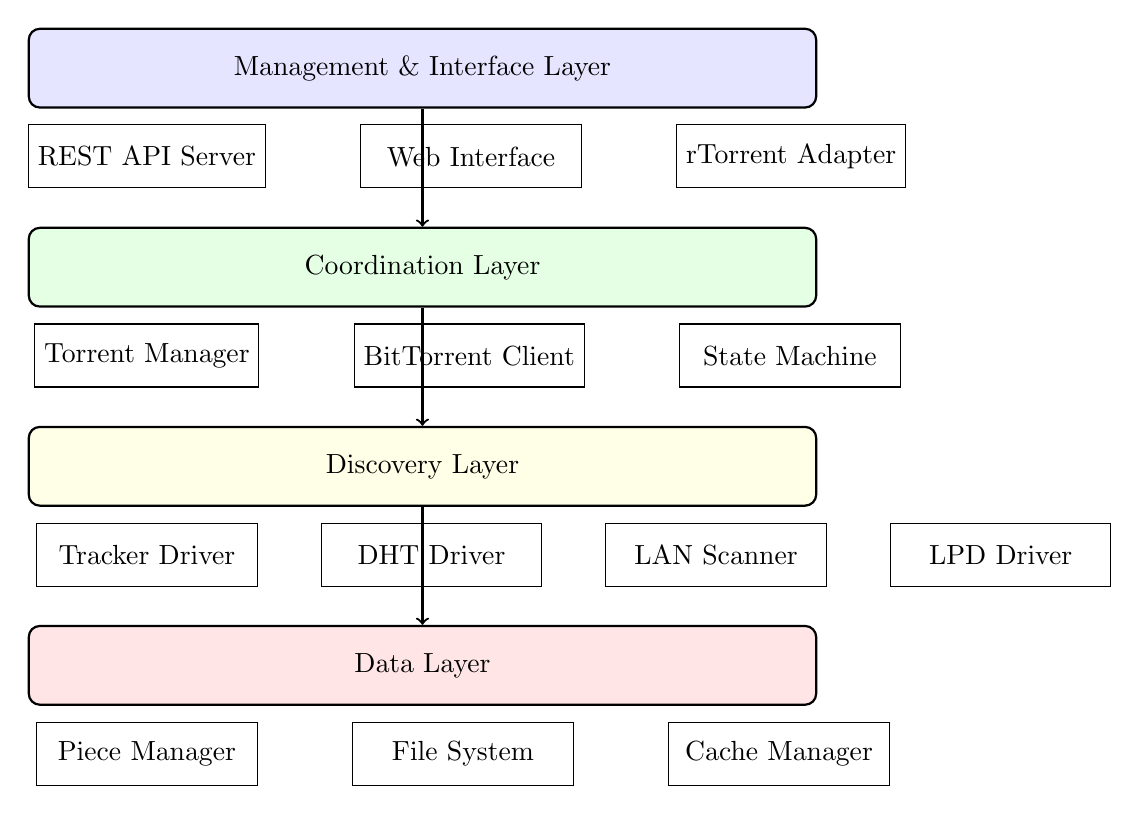
\begin{tikzpicture}[
    node distance=1cm,
    layer/.style={rectangle, draw=black, thick, minimum width=10cm, minimum height=1cm, align=center, rounded corners},
    component/.style={rectangle, draw=black, minimum width=2.8cm, minimum height=0.8cm, align=center}
]

% Management Layer
\node[layer, fill=blue!10] (management) {Management \& Interface Layer};
\node[component, below=0.2cm of management.south, xshift=-3.5cm] (api) {REST API Server};
\node[component, right=1.2cm of api] (web) {Web Interface};
\node[component, right=1.2cm of web] (compat) {rTorrent Adapter};

% Coordination Layer
\node[layer, fill=green!10, below=1.5cm of management] (coordination) {Coordination Layer};
\node[component, below=0.2cm of coordination.south, xshift=-3.5cm] (manager) {Torrent Manager};
\node[component, right=1.2cm of manager] (client) {BitTorrent Client};
\node[component, right=1.2cm of client] (state) {State Machine};

% Discovery Layer
\node[layer, fill=yellow!10, below=1.5cm of coordination] (discovery) {Discovery Layer};
\node[component, below=0.2cm of discovery.south, xshift=-3.5cm] (tracker) {Tracker Driver};
\node[component, right=0.8cm of tracker] (dht) {DHT Driver};
\node[component, right=0.8cm of dht] (lan) {LAN Scanner};
\node[component, right=0.8cm of lan] (lpd) {LPD Driver};

% Data Layer
\node[layer, fill=red!10, below=1.5cm of discovery] (data) {Data Layer};
\node[component, below=0.2cm of data.south, xshift=-3.5cm] (pieces) {Piece Manager};
\node[component, right=1.2cm of pieces] (files) {File System};
\node[component, right=1.2cm of files] (cache) {Cache Manager};

% Vertical connections
\draw[thick, ->] (management.south) -- (coordination.north);
\draw[thick, ->] (coordination.south) -- (discovery.north);
\draw[thick, ->] (discovery.south) -- (data.north);

\end{tikzpicture}
\caption{BlobTorrent's layered system architecture}
\end{figure}



The layered architecture represents a deliberate departure from monolithic client designs. Each layer specializes in a specific class of operations while maintaining clean interfaces to adjacent layers. This separation of concerns means that improvements to one layer don't require changes to others, and issues can be isolated and resolved without system-wide impact.

The \textbf{Control \& Interface Layer} handles all user and external system interactions, ensuring that the client remains responsive even during heavy background operations. The HTTP REST API and rTorrent adapter transform BlobTorrent from a standalone application into an integrable component that can participate in larger systems.

The \textbf{Core Coordination Layer} acts as the system's nervous system, managing the complex interplay between different components. This is where intelligent decisions about piece selection, peer management, and resource allocation happen. These are refered to as "Manager"s in the codebase. Managers handle port allocation, connections, pieces, \&c.

The \textbf{Network \& Discovery Layer} specializes in the challenging task of finding and maintaining connections in a dynamic, unreliable network environment. This layer's multi-method approach to peer discovery means that BlobTorrent can adapt to network conditions that would cripple single-method clients.

The \textbf{Data \& Storage Layer} optimizes the critical path between network reception and disk persistence. The block caching, managed I/O, and verification systems work together to ensure that data integrity is maintained without sacrificing performance.

\subsection{Concurrency Model: Right Tool for Each Task}

The hybrid concurrency model represents a pragmatic approach to managing simultaneous operations. Rather than forcing all tasks into a single concurrency paradigm, BlobTorrent matches the concurrency approach to the task characteristics.

Network I/O benefits from a thread pool model because these operations are naturally parallelizable and spend most of their time waiting for external responses. Disk operations similarly benefit from dedicated threads that can handle the blocking nature of filesystem interactions without impacting other system components.

Interface threads ensure that user interactions remain responsive regardless of background activity. This separation means that updating a progress display or handling API requests never waits for disk writes or network operations to complete.

In peer-to-peer communication, besides handling read and write operations in different threads, the system also makes use of a buffer to make full use of the available bandwith in low-latency environments. Bandwith consumption and waste is mitigated by a simple congestion protocol based on TCP's.

This thoughtful approach to concurrency means that BlobTorrent can scale to handle hundreds of simultaneous connections and multiple large downloads while remaining responsive and stable—a combination that eludes many traditional clients.

\section{Communication \& Localization: Finding the Swarm}

\subsection{The Peer Discovery Challenge in Modern Networks}

Finding peers in today's complex network environments presents challenges that didn't exist when BitTorrent was originally designed. The proliferation of NATs, firewalls, and network filtering means that traditional tracker-based discovery often fails entirely. Meanwhile, the ephemeral nature of many peers means that swarms can change composition completely within minutes.

Traditional clients approach this problem with a primary-replica mindset: try the main method (trackers) and fall back to secondary methods only when the primary fails. This approach creates several problems: slow initial discovery as clients wait for tracker timeouts, complete failure when multiple discovery methods encounter issues simultaneously, and inefficient use of available information sources.

BlobTorrent's multi-layered discovery strategy addresses these limitations by treating all discovery methods as first-class citizens that can work in parallel. This approach recognizes that different methods excel in different scenarios: trackers work well for initial discovery in healthy swarms \citep{bep0003}, DHT provides resilience when trackers fail \citep{bep0005}, local discovery optimizes for network-local peers, and cached peers enable rapid reconnection to known-good sources.

\subsection{The Monitoring Problem}

Even if it's a single instance managing a single torrent, or a distributed application serving petabytes of data, logs and statistics play a critical role in the lifecycle BlobTorrent. Statistics can be fetched at any time via the HTTP (UNIX socket support is planned) REST API; furthermore, an adapter can be used to integrate the back-end with any rTorrent-compatible front-end.
Each node comes with their own adapter for seamless integration with distirbuted services.
HTTPS support for additional security is planned. The adapter can be configured to use UNIX sockets.

\section{Coordination \& Intelligence: Managing the Swarm}

\subsection{The Swarm Management Complexity Problem}

Managing a BitTorrent swarm involves solving multiple interconnected optimization problems simultaneously. Traditional clients often use simplistic, static algorithms that fail to adapt to changing swarm conditions. This leads to suboptimal performance, poor resource utilization, and negative impacts on overall swarm health.

The core challenge lies in the dynamic, distributed nature of BitTorrent swarms. Peers join and leave constantly, network conditions change minute by minute, and piece availability shifts as downloads progress. Static algorithms that work well in one scenario may perform poorly in another. For example, rarest-first piece selection optimizes for swarm health but can perform poorly for streaming media, while sequential selection enables streaming but harms swarm efficiency.

While we know there is no such thing as a free lunch, most algorithms (namely the piece selection algorithm, congestion control algorithm) can be enhanced with hand-crafted, configurable heuristics to provide the best service for each use-case.

\subsection{State Machines: Managing Protocol Complexity}

The hierarchical state machine system addresses a fundamental problem in BitTorrent clients: protocol compliance while maintaining resilience. Traditional clients often use ad-hoc state management that can get stuck in inconsistent states or violate protocol specifications during edge cases.

BlobTorrent's state machines provide several key advantages. First, they ensure protocol compliance by explicitly defining valid state transitions and preventing invalid ones \citep{bep0003}. This is particularly important for interoperability with diverse client implementations, some of which may be strict about protocol adherence.

Second, the state machines enable graceful error recovery by providing clear paths from error states back to normal operation. When a connection fails or a protocol error occurs, the system knows exactly how to reset the connection and resume operations, rather than leaving connections in limbo or requiring manual intervention.

Third, the state machines make the system's behavior predictable and debuggable. By explicitly modeling all possible states and transitions, BlobTorrent avoids the unpredictable emergent behaviors that often plague complex concurrent systems.

\subsection{Adaptive Piece Selection: Beyond Basic Algorithms}

The piece selection system in BlobTorrent represents a significant advancement over traditional approaches by recognizing that different scenarios call for different strategies \citep{legout2007understanding}. The configurable selection framework allows BlobTorrent to optimize for specific use cases while maintaining the flexibility to adapt as conditions change.

Using the flexible soft-max function, and assigning dynamic weights for each set of requirements (rare pieces, low number of open files, secuential downloads)the client can adapt to many use-cases.

The endgame mode solves a notorious problem in BitTorrent downloads: the final slowdown. Traditional clients can take disproportionately long to download the last few pieces because they rely on a small number of peers that happen to have those pieces. BlobTorrent's aggressive endgame strategy requests all remaining blocks from all available peers, dramatically reducing completion time while intelligently canceling redundant requests to avoid wasting bandwidth \citep{bep0003}.
This is also paramount in hostile environments where we are recovering from a failure (bootstraping with the peer cache, for example) and most of the peers are not responding to requests, leading to starvation since the "bad peers" lock the last pieces and the "good peers" time out.

This adaptive approach to piece selection means that BlobTorrent consistently achieves faster download completion times while maintaining better swarm citizenship than clients with static algorithms.

\subsection{Congestion Control and Fairness: Network Citizenship}

The TCP-inspired congestion control system addresses a critical but often overlooked aspect of BitTorrent clients: network impact. Traditional clients can overwhelm network links, causing packet loss and performance degradation for all network users. This is particularly problematic in shared network environments like home networks, offices, and dormitories.

BlobTorrent's congestion control implements the same additive increase/multiplicative decrease algorithm used by TCP, ensuring that the client behaves as a good network citizen. This approach means that BlobTorrent shares bandwidth fairly with other TCP-based applications like web browsing, video streaming, and online gaming. The result is smoother overall network performance, fewer complaints from other network users.

\section{Data Integrity: Ensuring File Consistency}

\subsection{The Corruption Challenge in Distributed Systems}

In a system where data comes from potentially hundreds of untrusted sources across unreliable networks, ensuring file integrity is not just a feature—it's a fundamental requirement. Traditional approaches to integrity checking often create their own problems: full-file verification after interruptions is slow and I/O intensive, while insufficient verification can allow corrupted files to go undetected.

The challenge is particularly acute in BitTorrent because of the distributed nature of the data sources. A single malicious peer can inject corrupted blocks that, if undetected, could compromise entire downloads. Meanwhile, legitimate corruption can occur due to network errors, disk issues, or software bugs in other clients.

Data verification is a first-class feature of the BitTorrent protocol; no piece is written in disk without verification.

\subsection{State Persistence and Recovery}

The FastResume system addresses one of the most frustrating aspects of traditional BitTorrent clients: losing progress during restarts. BlobTorrent's mitigates this by caching both peers and downloaded blocks; this approach ensures nothing of value is lost during a crash or an interruption.

This comprehensive state capture means that restarts are truly seamless. When BlobTorrent resumes after a crash or planned shutdown, it can immediately reconnect to productive peers, resume downloads from the exact point of interruption, and continue downloading or serving data to peers.

The system's integrity checking for resume data is particularly important. By verifying that resume data hasn't been corrupted or tampered with, BlobTorrent prevents the nightmare scenario of resuming with corrupted state information that could lead to file corruption or wasted downloads.

This sophisticated approach to state management means that BlobTorrent users can have confidence that their downloads will survive system restarts, power outages, and client upgrades—a level of reliability that's essential for large downloads or situations with unreliable infrastructure.

\subsection{Disk I/O Optimization}

The managed file descriptor pool solves a practical but critical problem: operating system limits on open files. Traditional clients can exhaust these limits when handling many torrents with multiple files, leading to mysterious failures and corrupted downloads.

BlobTorrent's pool management uses LRU eviction to ensure that file descriptors are available when needed while preventing exhaustion.

\section{Security: Protection in a Hostile Environment}

\subsection{The Modern Threat Landscape}

\textbf{The Problem:} BitTorrent clients operate in one of the most hostile network environments imaginable \citep{wallach2006survey}. They must contend with malicious peers attempting to corrupt downloads, surveillance entities monitoring P2P traffic, ISP throttling targeting P2P protocols, and potential vulnerabilities in exposed management interfaces. Traditional clients often treat security as an afterthought, leaving users exposed to multiple attack vectors.

The threats are both technical and legal in nature. On the technical side, attackers can deploy eclipse attacks to isolate clients from legitimate peers, inject corrupted data to waste bandwidth and storage, or exploit vulnerabilities in protocol implementations. On the legal and operational side, ISPs increasingly deploy deep packet inspection to throttle or block BitTorrent traffic, while malicious entities may scan for exposed management interfaces.

\textbf{Our Solution:} None but the implementation of the corresponding BEPs is planned \citep{bep0042}...

\section{Usability \& Integration: Beyond the Command Line}

\subsection{The Management Complexity Problem}

\textbf{The Problem:} Traditional BitTorrent clients present a fundamental usability challenge: they must balance powerful, technical functionality with accessibility for non-technical users. This often results in either overwhelming complexity that alienates casual users or oversimplified interfaces that frustrate power users. Additionally, the growing need for remote management, automation, and integration with other systems creates requirements that traditional desktop-centric designs cannot satisfy.

The management challenge extends beyond the user interface to encompass deployment, monitoring, and maintenance. System administrators need centralized control over multiple client instances, developers require APIs for building custom applications, and home users want intuitive interfaces that work across all their devices. Traditional clients, designed as monolithic desktop applications, struggle to meet these diverse needs simultaneously.

\textbf{Our Solution:} BlobTorrent reimagines BitTorrent client usability through a multi-interface architecture that provides appropriate interaction models for different user types and use cases. The web-based interface offers modern accessibility, the comprehensive API enables automation and integration, and the rTorrent compatibility layer ensures smooth transition for existing users. This approach recognizes that usability isn't about finding a one-size-fits-all solution, but about providing the right tools for different contexts.

\subsection{Web Interface \& Visualization}

\subsubsection{Modern Web-Based Management}

\textbf{The Problem:} Desktop-bound interfaces limit accessibility and create deployment friction. Users increasingly expect to manage applications from any device, anywhere, without installing specialized software or configuring complex network access.

\textbf{Our Solution:} BlobTorrent's responsive web interface (or rather, rTorrent's responsive web interface: $flood$) provides full client functionality through any modern web browser, combining the power of a desktop application with the accessibility of web technology.

\subsection{HTTP REST API Ecosystem}

\subsubsection{Comprehensive Programmatic Interface}

\textbf{The Problem:} Automation and integration require stable, well-documented APIs that expose all client functionality. Traditional clients often provide limited scripting interfaces or unstable internal APIs that break between versions.

\textbf{Our Solution:} BlobTorrent's HTTP REST API offers complete, versioned access to all client features through a consistent, well-documented interface designed for both simple automation and complex integration scenarios.

The API design follows RESTful principles with predictable resource naming, standard HTTP methods, and consistent error handling. All operations are available through the API, from basic torrent management to advanced configuration and real-time monitoring. The versioning strategy ensures that integrations continue working across client updates, while new features become available through explicit version selection.

\subsection{rTorrent Compatibility Layer}

\subsubsection{Seamless Ecosystem Migration}

\textbf{The Problem:} Existing rTorrent users have significant investment in configured systems, custom scripts, and workflow familiarity. Migrating to a new client often means abandoning this investment and relearning established workflows.

\textbf{Our Solution:} BlobTorrent's rTorrent compatibility layer provides near-perfect protocol compatibility, allowing existing rTorrent front-ends, scripts, and configurations to work unchanged while gaining BlobTorrent's modern architecture and enhanced capabilities.

The compatibility layer operates at multiple levels. At the protocol level, it implements the exact XML-RPC interface that rTorrent exposes, supporting all methods and data formats. Existing front-ends like Flood, ruTorrent, and pyrocore connect to BlobTorrent exactly as they would to rTorrent, without modification or configuration changes.

For script and automation compatibility, the layer supports rTorrent's event system and command execution patterns. Existing scripts that handle download completion, schedule-based actions, or custom notifications continue working without modification. This is particularly valuable for users with complex post-processing workflows or integration with other systems through rTorrent's extensibility mechanisms.

\bibliographystyle{plainnat}
\bibliography{references}

\end{document}
